% Created by tikzDevice version 0.12.3.1 on 2022-04-28 16:23:10
% !TEX encoding = UTF-8 Unicode
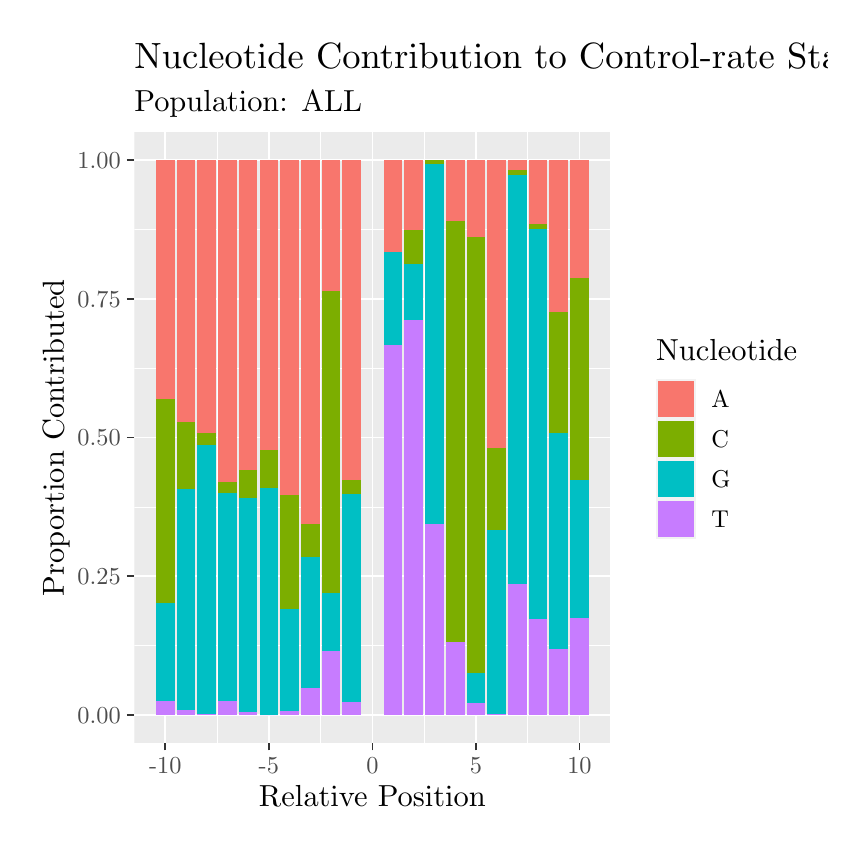
\begin{tikzpicture}[x=1pt,y=1pt]
\definecolor{fillColor}{RGB}{255,255,255}
\path[use as bounding box,fill=fillColor,fill opacity=0.00] (0,0) rectangle (289.08,289.08);
\begin{scope}
\path[clip] (  0.00,  0.00) rectangle (289.08,289.08);
\definecolor{drawColor}{RGB}{255,255,255}
\definecolor{fillColor}{RGB}{255,255,255}

\path[draw=drawColor,line width= 0.6pt,line join=round,line cap=round,fill=fillColor] (  0.00,  0.00) rectangle (289.08,289.08);
\end{scope}
\begin{scope}
\path[clip] ( 38.56, 30.69) rectangle (210.56,251.21);
\definecolor{fillColor}{gray}{0.92}

\path[fill=fillColor] ( 38.56, 30.69) rectangle (210.56,251.21);
\definecolor{drawColor}{RGB}{255,255,255}

\path[draw=drawColor,line width= 0.3pt,line join=round] ( 38.56, 65.77) --
	(210.56, 65.77);

\path[draw=drawColor,line width= 0.3pt,line join=round] ( 38.56,115.89) --
	(210.56,115.89);

\path[draw=drawColor,line width= 0.3pt,line join=round] ( 38.56,166.01) --
	(210.56,166.01);

\path[draw=drawColor,line width= 0.3pt,line join=round] ( 38.56,216.13) --
	(210.56,216.13);

\path[draw=drawColor,line width= 0.3pt,line join=round] ( 68.45, 30.69) --
	( 68.45,251.21);

\path[draw=drawColor,line width= 0.3pt,line join=round] (105.85, 30.69) --
	(105.85,251.21);

\path[draw=drawColor,line width= 0.3pt,line join=round] (143.26, 30.69) --
	(143.26,251.21);

\path[draw=drawColor,line width= 0.3pt,line join=round] (180.67, 30.69) --
	(180.67,251.21);

\path[draw=drawColor,line width= 0.6pt,line join=round] ( 38.56, 40.71) --
	(210.56, 40.71);

\path[draw=drawColor,line width= 0.6pt,line join=round] ( 38.56, 90.83) --
	(210.56, 90.83);

\path[draw=drawColor,line width= 0.6pt,line join=round] ( 38.56,140.95) --
	(210.56,140.95);

\path[draw=drawColor,line width= 0.6pt,line join=round] ( 38.56,191.07) --
	(210.56,191.07);

\path[draw=drawColor,line width= 0.6pt,line join=round] ( 38.56,241.18) --
	(210.56,241.18);

\path[draw=drawColor,line width= 0.6pt,line join=round] ( 49.74, 30.69) --
	( 49.74,251.21);

\path[draw=drawColor,line width= 0.6pt,line join=round] ( 87.15, 30.69) --
	( 87.15,251.21);

\path[draw=drawColor,line width= 0.6pt,line join=round] (124.56, 30.69) --
	(124.56,251.21);

\path[draw=drawColor,line width= 0.6pt,line join=round] (161.97, 30.69) --
	(161.97,251.21);

\path[draw=drawColor,line width= 0.6pt,line join=round] (199.38, 30.69) --
	(199.38,251.21);
\definecolor{fillColor}{RGB}{248,118,109}

\path[fill=fillColor] ( 46.37,154.90) rectangle ( 53.11,241.18);
\definecolor{fillColor}{RGB}{124,174,0}

\path[fill=fillColor] ( 46.37, 81.26) rectangle ( 53.11,154.90);
\definecolor{fillColor}{RGB}{199,124,255}

\path[fill=fillColor] ( 46.37, 40.71) rectangle ( 53.11, 45.87);
\definecolor{fillColor}{RGB}{0,191,196}

\path[fill=fillColor] ( 46.37, 45.87) rectangle ( 53.11, 81.26);
\definecolor{fillColor}{RGB}{248,118,109}

\path[fill=fillColor] ( 53.86,146.70) rectangle ( 60.59,241.18);
\definecolor{fillColor}{RGB}{124,174,0}

\path[fill=fillColor] ( 53.86,122.25) rectangle ( 60.59,146.70);
\definecolor{fillColor}{RGB}{0,191,196}

\path[fill=fillColor] ( 53.86, 42.62) rectangle ( 60.59,122.25);
\definecolor{fillColor}{RGB}{199,124,255}

\path[fill=fillColor] ( 53.86, 40.71) rectangle ( 60.59, 42.62);
\definecolor{fillColor}{RGB}{248,118,109}

\path[fill=fillColor] ( 61.34,142.47) rectangle ( 68.07,241.18);
\definecolor{fillColor}{RGB}{124,174,0}

\path[fill=fillColor] ( 61.34,138.22) rectangle ( 68.07,142.47);
\definecolor{fillColor}{RGB}{199,124,255}

\path[fill=fillColor] ( 61.34, 40.71) rectangle ( 68.07, 40.95);
\definecolor{fillColor}{RGB}{0,191,196}

\path[fill=fillColor] ( 61.34, 40.95) rectangle ( 68.07,138.22);
\definecolor{fillColor}{RGB}{248,118,109}

\path[fill=fillColor] ( 68.82,124.77) rectangle ( 75.55,241.18);
\definecolor{fillColor}{RGB}{124,174,0}

\path[fill=fillColor] ( 68.82,120.91) rectangle ( 75.55,124.77);
\definecolor{fillColor}{RGB}{199,124,255}

\path[fill=fillColor] ( 68.82, 40.71) rectangle ( 75.55, 45.78);
\definecolor{fillColor}{RGB}{0,191,196}

\path[fill=fillColor] ( 68.82, 45.78) rectangle ( 75.55,120.91);
\definecolor{fillColor}{RGB}{248,118,109}

\path[fill=fillColor] ( 76.30,129.42) rectangle ( 83.04,241.18);
\definecolor{fillColor}{RGB}{124,174,0}

\path[fill=fillColor] ( 76.30,119.11) rectangle ( 83.04,129.42);
\definecolor{fillColor}{RGB}{199,124,255}

\path[fill=fillColor] ( 76.30, 40.71) rectangle ( 83.04, 41.85);
\definecolor{fillColor}{RGB}{0,191,196}

\path[fill=fillColor] ( 76.30, 41.85) rectangle ( 83.04,119.11);
\definecolor{fillColor}{RGB}{248,118,109}

\path[fill=fillColor] ( 83.78,136.43) rectangle ( 90.52,241.18);
\definecolor{fillColor}{RGB}{124,174,0}

\path[fill=fillColor] ( 83.78,122.86) rectangle ( 90.52,136.43);
\definecolor{fillColor}{RGB}{0,191,196}

\path[fill=fillColor] ( 83.78, 40.71) rectangle ( 90.52,122.86);
\definecolor{fillColor}{RGB}{199,124,255}

\path[fill=fillColor] ( 83.78, 40.71) rectangle ( 90.52, 40.71);
\definecolor{fillColor}{RGB}{248,118,109}

\path[fill=fillColor] ( 91.27,120.36) rectangle ( 98.00,241.18);
\definecolor{fillColor}{RGB}{124,174,0}

\path[fill=fillColor] ( 91.27, 79.04) rectangle ( 98.00,120.36);
\definecolor{fillColor}{RGB}{0,191,196}

\path[fill=fillColor] ( 91.27, 42.22) rectangle ( 98.00, 79.04);
\definecolor{fillColor}{RGB}{199,124,255}

\path[fill=fillColor] ( 91.27, 40.71) rectangle ( 98.00, 42.22);
\definecolor{fillColor}{RGB}{248,118,109}

\path[fill=fillColor] ( 98.75,109.90) rectangle (105.48,241.18);
\definecolor{fillColor}{RGB}{124,174,0}

\path[fill=fillColor] ( 98.75, 97.71) rectangle (105.48,109.90);
\definecolor{fillColor}{RGB}{0,191,196}

\path[fill=fillColor] ( 98.75, 50.47) rectangle (105.48, 97.71);
\definecolor{fillColor}{RGB}{199,124,255}

\path[fill=fillColor] ( 98.75, 40.71) rectangle (105.48, 50.47);
\definecolor{fillColor}{RGB}{248,118,109}

\path[fill=fillColor] (106.23,194.01) rectangle (112.96,241.18);
\definecolor{fillColor}{RGB}{124,174,0}

\path[fill=fillColor] (106.23, 84.69) rectangle (112.96,194.01);
\definecolor{fillColor}{RGB}{0,191,196}

\path[fill=fillColor] (106.23, 63.98) rectangle (112.96, 84.69);
\definecolor{fillColor}{RGB}{199,124,255}

\path[fill=fillColor] (106.23, 40.71) rectangle (112.96, 63.98);
\definecolor{fillColor}{RGB}{248,118,109}

\path[fill=fillColor] (113.71,125.77) rectangle (120.44,241.18);
\definecolor{fillColor}{RGB}{124,174,0}

\path[fill=fillColor] (113.71,120.63) rectangle (120.44,125.77);
\definecolor{fillColor}{RGB}{199,124,255}

\path[fill=fillColor] (113.71, 40.71) rectangle (120.44, 45.47);
\definecolor{fillColor}{RGB}{0,191,196}

\path[fill=fillColor] (113.71, 45.47) rectangle (120.44,120.63);
\definecolor{fillColor}{RGB}{248,118,109}

\path[fill=fillColor] (128.67,208.19) rectangle (135.41,241.18);
\definecolor{fillColor}{RGB}{124,174,0}

\path[fill=fillColor] (128.67,208.14) rectangle (135.41,208.19);
\definecolor{fillColor}{RGB}{0,191,196}

\path[fill=fillColor] (128.67,174.39) rectangle (135.41,208.14);
\definecolor{fillColor}{RGB}{199,124,255}

\path[fill=fillColor] (128.67, 40.71) rectangle (135.41,174.39);
\definecolor{fillColor}{RGB}{248,118,109}

\path[fill=fillColor] (136.16,215.84) rectangle (142.89,241.18);
\definecolor{fillColor}{RGB}{124,174,0}

\path[fill=fillColor] (136.16,203.56) rectangle (142.89,215.84);
\definecolor{fillColor}{RGB}{0,191,196}

\path[fill=fillColor] (136.16,183.40) rectangle (142.89,203.56);
\definecolor{fillColor}{RGB}{199,124,255}

\path[fill=fillColor] (136.16, 40.71) rectangle (142.89,183.40);
\definecolor{fillColor}{RGB}{248,118,109}

\path[fill=fillColor] (143.64,241.16) rectangle (150.37,241.18);
\definecolor{fillColor}{RGB}{124,174,0}

\path[fill=fillColor] (143.64,239.83) rectangle (150.37,241.16);
\definecolor{fillColor}{RGB}{0,191,196}

\path[fill=fillColor] (143.64,109.64) rectangle (150.37,239.83);
\definecolor{fillColor}{RGB}{199,124,255}

\path[fill=fillColor] (143.64, 40.71) rectangle (150.37,109.64);
\definecolor{fillColor}{RGB}{248,118,109}

\path[fill=fillColor] (151.12,219.13) rectangle (157.85,241.18);
\definecolor{fillColor}{RGB}{124,174,0}

\path[fill=fillColor] (151.12, 66.92) rectangle (157.85,219.13);
\definecolor{fillColor}{RGB}{0,191,196}

\path[fill=fillColor] (151.12, 66.92) rectangle (157.85, 66.92);
\definecolor{fillColor}{RGB}{199,124,255}

\path[fill=fillColor] (151.12, 40.71) rectangle (157.85, 66.92);
\definecolor{fillColor}{RGB}{248,118,109}

\path[fill=fillColor] (158.60,213.33) rectangle (165.34,241.18);
\definecolor{fillColor}{RGB}{124,174,0}

\path[fill=fillColor] (158.60, 55.97) rectangle (165.34,213.33);
\definecolor{fillColor}{RGB}{0,191,196}

\path[fill=fillColor] (158.60, 45.08) rectangle (165.34, 55.97);
\definecolor{fillColor}{RGB}{199,124,255}

\path[fill=fillColor] (158.60, 40.71) rectangle (165.34, 45.08);
\definecolor{fillColor}{RGB}{248,118,109}

\path[fill=fillColor] (166.08,137.27) rectangle (172.82,241.18);
\definecolor{fillColor}{RGB}{124,174,0}

\path[fill=fillColor] (166.08,107.73) rectangle (172.82,137.27);
\definecolor{fillColor}{RGB}{0,191,196}

\path[fill=fillColor] (166.08, 41.02) rectangle (172.82,107.73);
\definecolor{fillColor}{RGB}{199,124,255}

\path[fill=fillColor] (166.08, 40.71) rectangle (172.82, 41.02);
\definecolor{fillColor}{RGB}{248,118,109}

\path[fill=fillColor] (173.57,237.63) rectangle (180.30,241.18);
\definecolor{fillColor}{RGB}{124,174,0}

\path[fill=fillColor] (173.57,235.74) rectangle (180.30,237.63);
\definecolor{fillColor}{RGB}{0,191,196}

\path[fill=fillColor] (173.57, 87.96) rectangle (180.30,235.74);
\definecolor{fillColor}{RGB}{199,124,255}

\path[fill=fillColor] (173.57, 40.71) rectangle (180.30, 87.96);
\definecolor{fillColor}{RGB}{248,118,109}

\path[fill=fillColor] (181.05,218.06) rectangle (187.78,241.18);
\definecolor{fillColor}{RGB}{124,174,0}

\path[fill=fillColor] (181.05,216.44) rectangle (187.78,218.06);
\definecolor{fillColor}{RGB}{0,191,196}

\path[fill=fillColor] (181.05, 75.58) rectangle (187.78,216.44);
\definecolor{fillColor}{RGB}{199,124,255}

\path[fill=fillColor] (181.05, 40.71) rectangle (187.78, 75.58);
\definecolor{fillColor}{RGB}{248,118,109}

\path[fill=fillColor] (188.53,186.23) rectangle (195.26,241.18);
\definecolor{fillColor}{RGB}{124,174,0}

\path[fill=fillColor] (188.53,142.65) rectangle (195.26,186.23);
\definecolor{fillColor}{RGB}{0,191,196}

\path[fill=fillColor] (188.53, 64.71) rectangle (195.26,142.65);
\definecolor{fillColor}{RGB}{199,124,255}

\path[fill=fillColor] (188.53, 40.71) rectangle (195.26, 64.71);
\definecolor{fillColor}{RGB}{248,118,109}

\path[fill=fillColor] (196.01,198.51) rectangle (202.75,241.18);
\definecolor{fillColor}{RGB}{124,174,0}

\path[fill=fillColor] (196.01,125.79) rectangle (202.75,198.51);
\definecolor{fillColor}{RGB}{199,124,255}

\path[fill=fillColor] (196.01, 40.71) rectangle (202.75, 75.83);
\definecolor{fillColor}{RGB}{0,191,196}

\path[fill=fillColor] (196.01, 75.83) rectangle (202.75,125.79);
\end{scope}
\begin{scope}
\path[clip] (  0.00,  0.00) rectangle (289.08,289.08);
\definecolor{drawColor}{gray}{0.30}

\node[text=drawColor,anchor=base east,inner sep=0pt, outer sep=0pt, scale=  0.88] at ( 33.61, 37.68) {0.00};

\node[text=drawColor,anchor=base east,inner sep=0pt, outer sep=0pt, scale=  0.88] at ( 33.61, 87.80) {0.25};

\node[text=drawColor,anchor=base east,inner sep=0pt, outer sep=0pt, scale=  0.88] at ( 33.61,137.92) {0.50};

\node[text=drawColor,anchor=base east,inner sep=0pt, outer sep=0pt, scale=  0.88] at ( 33.61,188.04) {0.75};

\node[text=drawColor,anchor=base east,inner sep=0pt, outer sep=0pt, scale=  0.88] at ( 33.61,238.15) {1.00};
\end{scope}
\begin{scope}
\path[clip] (  0.00,  0.00) rectangle (289.08,289.08);
\definecolor{drawColor}{gray}{0.20}

\path[draw=drawColor,line width= 0.6pt,line join=round] ( 35.81, 40.71) --
	( 38.56, 40.71);

\path[draw=drawColor,line width= 0.6pt,line join=round] ( 35.81, 90.83) --
	( 38.56, 90.83);

\path[draw=drawColor,line width= 0.6pt,line join=round] ( 35.81,140.95) --
	( 38.56,140.95);

\path[draw=drawColor,line width= 0.6pt,line join=round] ( 35.81,191.07) --
	( 38.56,191.07);

\path[draw=drawColor,line width= 0.6pt,line join=round] ( 35.81,241.18) --
	( 38.56,241.18);
\end{scope}
\begin{scope}
\path[clip] (  0.00,  0.00) rectangle (289.08,289.08);
\definecolor{drawColor}{gray}{0.20}

\path[draw=drawColor,line width= 0.6pt,line join=round] ( 49.74, 27.94) --
	( 49.74, 30.69);

\path[draw=drawColor,line width= 0.6pt,line join=round] ( 87.15, 27.94) --
	( 87.15, 30.69);

\path[draw=drawColor,line width= 0.6pt,line join=round] (124.56, 27.94) --
	(124.56, 30.69);

\path[draw=drawColor,line width= 0.6pt,line join=round] (161.97, 27.94) --
	(161.97, 30.69);

\path[draw=drawColor,line width= 0.6pt,line join=round] (199.38, 27.94) --
	(199.38, 30.69);
\end{scope}
\begin{scope}
\path[clip] (  0.00,  0.00) rectangle (289.08,289.08);
\definecolor{drawColor}{gray}{0.30}

\node[text=drawColor,anchor=base,inner sep=0pt, outer sep=0pt, scale=  0.88] at ( 49.74, 19.68) {-10};

\node[text=drawColor,anchor=base,inner sep=0pt, outer sep=0pt, scale=  0.88] at ( 87.15, 19.68) {-5};

\node[text=drawColor,anchor=base,inner sep=0pt, outer sep=0pt, scale=  0.88] at (124.56, 19.68) {0};

\node[text=drawColor,anchor=base,inner sep=0pt, outer sep=0pt, scale=  0.88] at (161.97, 19.68) {5};

\node[text=drawColor,anchor=base,inner sep=0pt, outer sep=0pt, scale=  0.88] at (199.38, 19.68) {10};
\end{scope}
\begin{scope}
\path[clip] (  0.00,  0.00) rectangle (289.08,289.08);
\definecolor{drawColor}{RGB}{0,0,0}

\node[text=drawColor,anchor=base,inner sep=0pt, outer sep=0pt, scale=  1.10] at (124.56,  7.64) {Relative Position};
\end{scope}
\begin{scope}
\path[clip] (  0.00,  0.00) rectangle (289.08,289.08);
\definecolor{drawColor}{RGB}{0,0,0}

\node[text=drawColor,rotate= 90.00,anchor=base,inner sep=0pt, outer sep=0pt, scale=  1.10] at ( 13.08,140.95) {Proportion Contributed};
\end{scope}
\begin{scope}
\path[clip] (  0.00,  0.00) rectangle (289.08,289.08);
\definecolor{fillColor}{RGB}{255,255,255}

\path[fill=fillColor] (221.56, 98.93) rectangle (283.58,182.96);
\end{scope}
\begin{scope}
\path[clip] (  0.00,  0.00) rectangle (289.08,289.08);
\definecolor{drawColor}{RGB}{0,0,0}

\node[text=drawColor,anchor=base west,inner sep=0pt, outer sep=0pt, scale=  1.10] at (227.06,168.82) {Nucleotide};
\end{scope}
\begin{scope}
\path[clip] (  0.00,  0.00) rectangle (289.08,289.08);
\definecolor{fillColor}{gray}{0.95}

\path[fill=fillColor] (227.06,147.79) rectangle (241.52,162.25);
\end{scope}
\begin{scope}
\path[clip] (  0.00,  0.00) rectangle (289.08,289.08);
\definecolor{fillColor}{RGB}{248,118,109}

\path[fill=fillColor] (227.78,148.51) rectangle (240.81,161.54);
\end{scope}
\begin{scope}
\path[clip] (  0.00,  0.00) rectangle (289.08,289.08);
\definecolor{fillColor}{gray}{0.95}

\path[fill=fillColor] (227.06,133.34) rectangle (241.52,147.79);
\end{scope}
\begin{scope}
\path[clip] (  0.00,  0.00) rectangle (289.08,289.08);
\definecolor{fillColor}{RGB}{124,174,0}

\path[fill=fillColor] (227.78,134.05) rectangle (240.81,147.08);
\end{scope}
\begin{scope}
\path[clip] (  0.00,  0.00) rectangle (289.08,289.08);
\definecolor{fillColor}{gray}{0.95}

\path[fill=fillColor] (227.06,118.89) rectangle (241.52,133.34);
\end{scope}
\begin{scope}
\path[clip] (  0.00,  0.00) rectangle (289.08,289.08);
\definecolor{fillColor}{RGB}{0,191,196}

\path[fill=fillColor] (227.78,119.60) rectangle (240.81,132.63);
\end{scope}
\begin{scope}
\path[clip] (  0.00,  0.00) rectangle (289.08,289.08);
\definecolor{fillColor}{gray}{0.95}

\path[fill=fillColor] (227.06,104.43) rectangle (241.52,118.89);
\end{scope}
\begin{scope}
\path[clip] (  0.00,  0.00) rectangle (289.08,289.08);
\definecolor{fillColor}{RGB}{199,124,255}

\path[fill=fillColor] (227.78,105.14) rectangle (240.81,118.17);
\end{scope}
\begin{scope}
\path[clip] (  0.00,  0.00) rectangle (289.08,289.08);
\definecolor{drawColor}{RGB}{0,0,0}

\node[text=drawColor,anchor=base west,inner sep=0pt, outer sep=0pt, scale=  0.88] at (247.02,151.99) {A};
\end{scope}
\begin{scope}
\path[clip] (  0.00,  0.00) rectangle (289.08,289.08);
\definecolor{drawColor}{RGB}{0,0,0}

\node[text=drawColor,anchor=base west,inner sep=0pt, outer sep=0pt, scale=  0.88] at (247.02,137.54) {C};
\end{scope}
\begin{scope}
\path[clip] (  0.00,  0.00) rectangle (289.08,289.08);
\definecolor{drawColor}{RGB}{0,0,0}

\node[text=drawColor,anchor=base west,inner sep=0pt, outer sep=0pt, scale=  0.88] at (247.02,123.08) {G};
\end{scope}
\begin{scope}
\path[clip] (  0.00,  0.00) rectangle (289.08,289.08);
\definecolor{drawColor}{RGB}{0,0,0}

\node[text=drawColor,anchor=base west,inner sep=0pt, outer sep=0pt, scale=  0.88] at (247.02,108.63) {T};
\end{scope}
\begin{scope}
\path[clip] (  0.00,  0.00) rectangle (289.08,289.08);
\definecolor{drawColor}{RGB}{0,0,0}

\node[text=drawColor,anchor=base west,inner sep=0pt, outer sep=0pt, scale=  1.10] at ( 38.56,258.85) {Population: ALL};
\end{scope}
\begin{scope}
\path[clip] (  0.00,  0.00) rectangle (289.08,289.08);
\definecolor{drawColor}{RGB}{0,0,0}

\node[text=drawColor,anchor=base west,inner sep=0pt, outer sep=0pt, scale=  1.32] at ( 38.56,274.49) {Nucleotide Contribution to Control-rate Statistic: AT-TA};
\end{scope}
\end{tikzpicture}
